\chapter{ITOLAB MOTORDRIVER}

\section{ドライバの特徴}
ITOLAB MOTORDRIVERを図\ref{fig:driver}に,回路図を図\ref{fig:dra}に示す.また,
ITOLAB MOTORDRIVERの仕様を表\ref{tab:shiyou}に示す.
ロボコンでは,ロボットに使用できる部品の上限価格が設定されている.今年度の上限は30万円で
ロボットを三台作製しなければならなかった.
また,作製するロボットに自動走行させたかったので,フィードバック制御が必要だった.

そこで,エンコーダが使用でき,製作コストが安いITOLAB MOTORDRIVERを使用することにした。

\begin{figure}[H]
  \begin{center}
    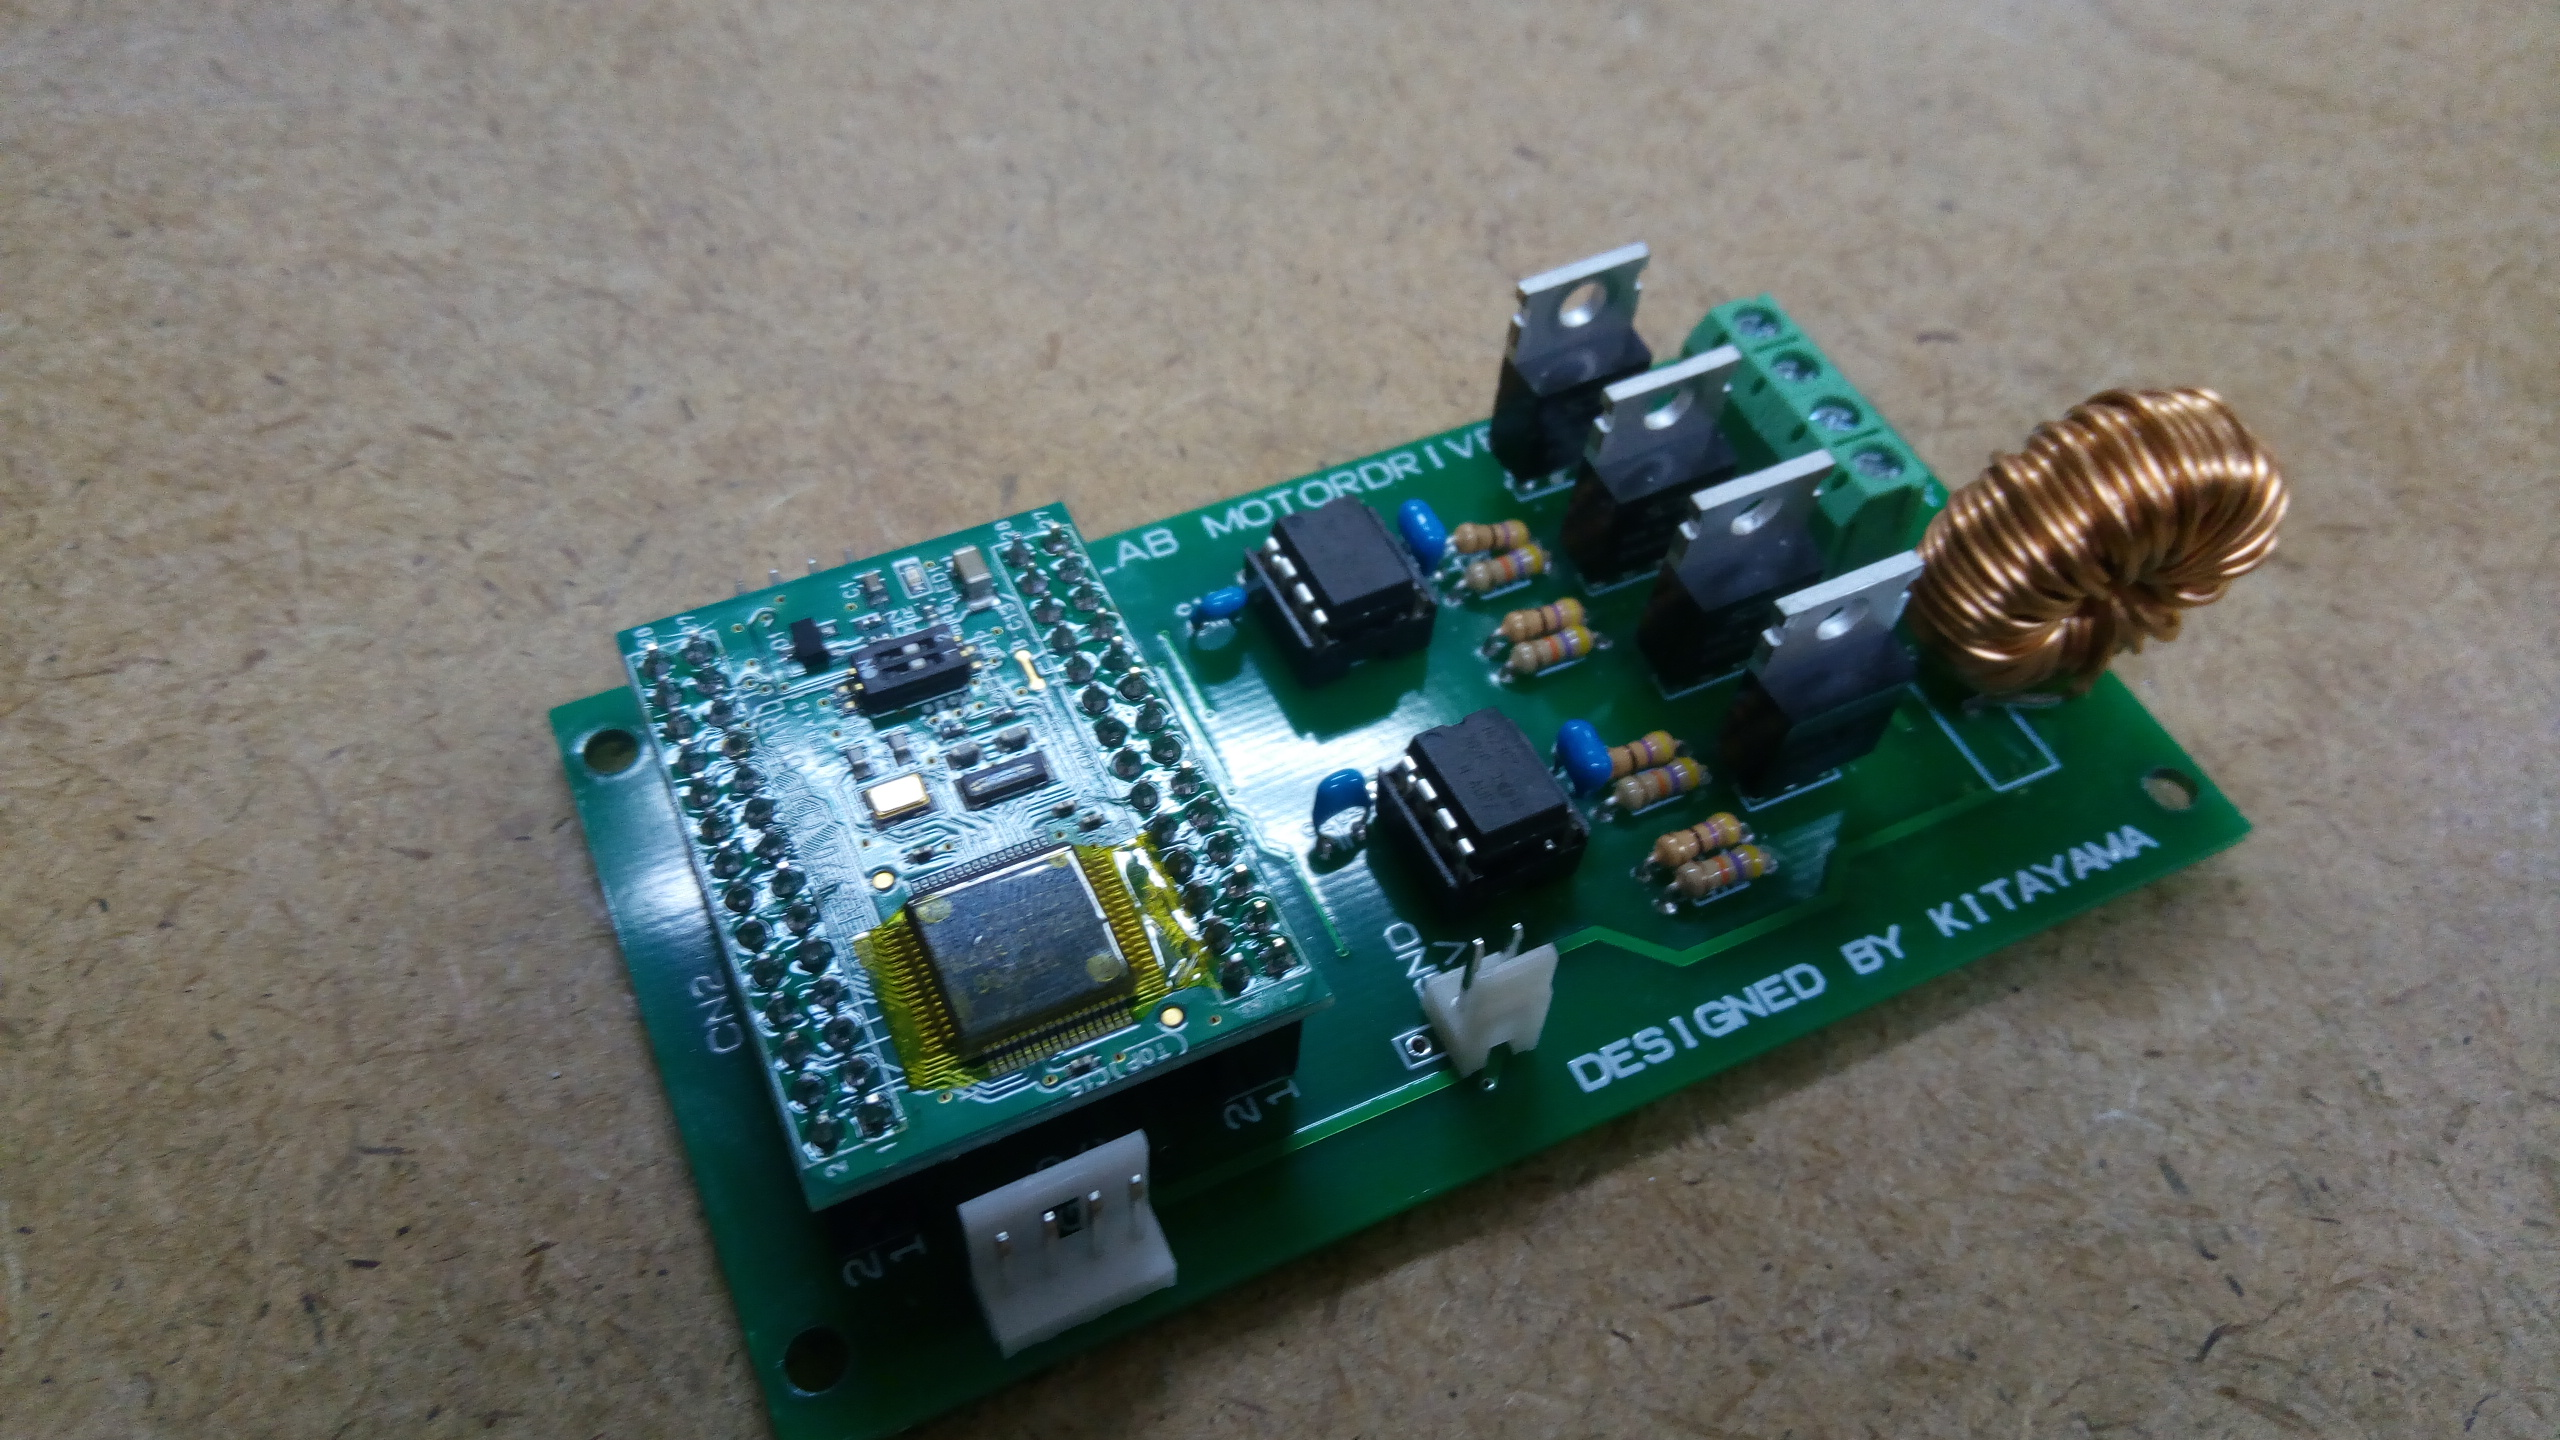
\includegraphics[width=150mm]{driver}
    \end{center}
  \caption{ITOLAB MOTORDRIVER}
 \label{fig:driver}
\end{figure}
\begin{figure}[H]
  \begin{center}
    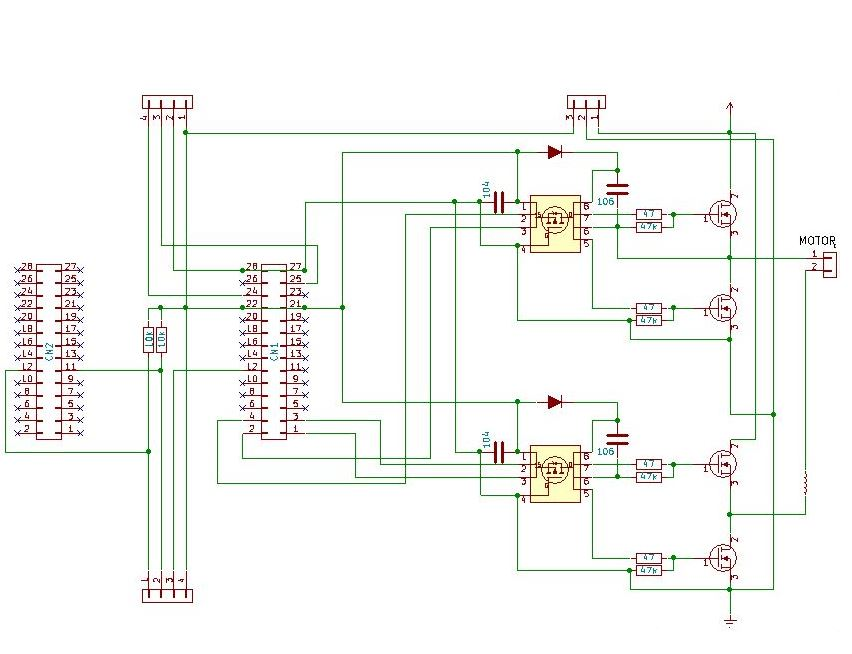
\includegraphics[width=150mm]{dra}
    \end{center}
  \caption{ITOLAB MOTORDRIVER回路図}
 \label{fig:dra}
\end{figure}
\begin{table}[htb]
\centering
\caption{ITOLAB MOTORDRIVERの仕様}
\begin{tabular}{|c|c|} \hline
使用マイコン&RX220マイコン\\ \hline
シリアル通信&RS232C\\ \hline
FET&$V_{DS}$  40V\\
   &$I_D$  80A\\ \hline
\end{tabular}
\label{tab:shiyou}
\end{table}

\section{改善点}
\subsection{発生した問題}
ロボットの動作実験を行うと,ITOLAB MOTORDRIVERに以下の問題が発生した.
\begin{itemize}
\item 急加減速時にパターンの焼損
\item 回生電流によるノイズの発生
\item FETトランジスタの高温化
\item 通信エラー
\end{itemize}
\subsubsection{パターンの焼損}
ロボットの走行実験中,ロボットを急加減速させた結果ロボット足回りから煙が上がり,
図\ref{fig:yake3}のようにモータドライバのパターンが焼損した.再現実験によりパターン
を焼損させた状態を図\ref{fig:jikkenn}に示す.
\begin{figure}[H]
  \begin{center}
    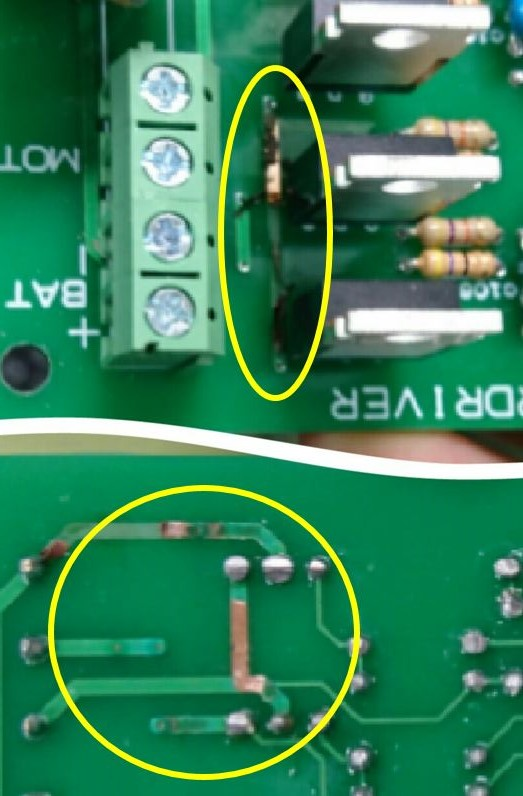
\includegraphics[width=100mm]{yake3}
    \end{center}
  \caption{パターンの焼損}
 \label{fig:yake3}
\end{figure}
\begin{figure}[H]
  \begin{center}
    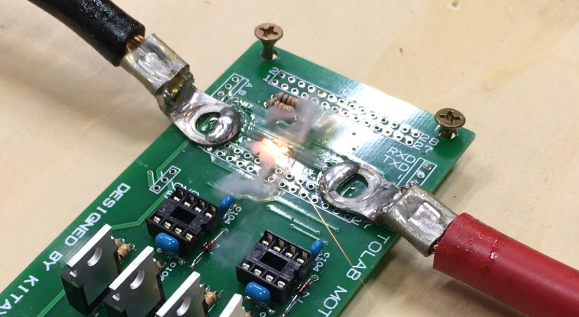
\includegraphics[width=100mm]{jikkenn}
    \end{center}
  \caption{実験によるパターンの焼損直後}
 \label{fig:jikkenn}
\end{figure}
\subsubsection{回生電流によるノイズの発生}
ロボットの走行実験中,ロボットを急加減速させた結果モータから回生電流が発生し,
ノイズとなった.
\subsubsection{FETトランジスタの高熱化}
移動速度が早いために,ロボットの前進,後進を繰り返した際電気エネルギが熱エネルギとなり,
FETトランジスタから高熱が発生された.
\subsubsection{通信エラー}
回生電流で発生したノイズによって,RS232C通信にノイズが乗り急停止時にロボットが暴走した.

\subsection{問題に対しての改善}
これらを解決するために,以下の対策を講じた.
改善後のITOLAB MOTORDRIVERを図\ref{fig:shin_driver}に,ロボットに取り付けた
ITOLAB MOTORDRIVERを図\ref{fig:robotuke}に示す.
\begin{itemize}
\item 電流制限プログラムの作成
\item 回生ダイオードの取り付け
\item FETトランジスタにヒートシンクの取り付け
\item 通信エラー確認用のLEDの取り付け
\end{itemize}
\subsubsection{電流制限プログラムの作成}
急加減速をするとパターンの焼損するので,プログラムで加減速を緩やかにして最高速度を
下げた.
\subsubsection{回生ダイオードの取り付け}
図\ref{fig:kai}の回生ダイオードを取り付けることで,モータから発生する回生電流から基板
を守り,ノイズを防ぐ.
\begin{figure}[H]
  \begin{center}
    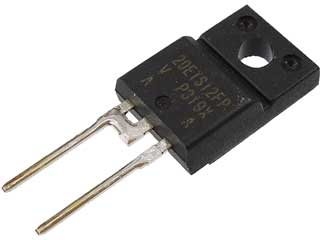
\includegraphics[width=50mm]{kai}
    \end{center}
  \caption{回生ダイオード}
 \label{fig:kai}
\end{figure}
\subsubsection{FETトランジスタにヒートシンクの取り付け}
ロボット操作によってFETで発生した熱を,図\ref{fig:hi-to}のヒートシンクで放熱,冷却する.
\begin{figure}[H]
  \begin{center}
    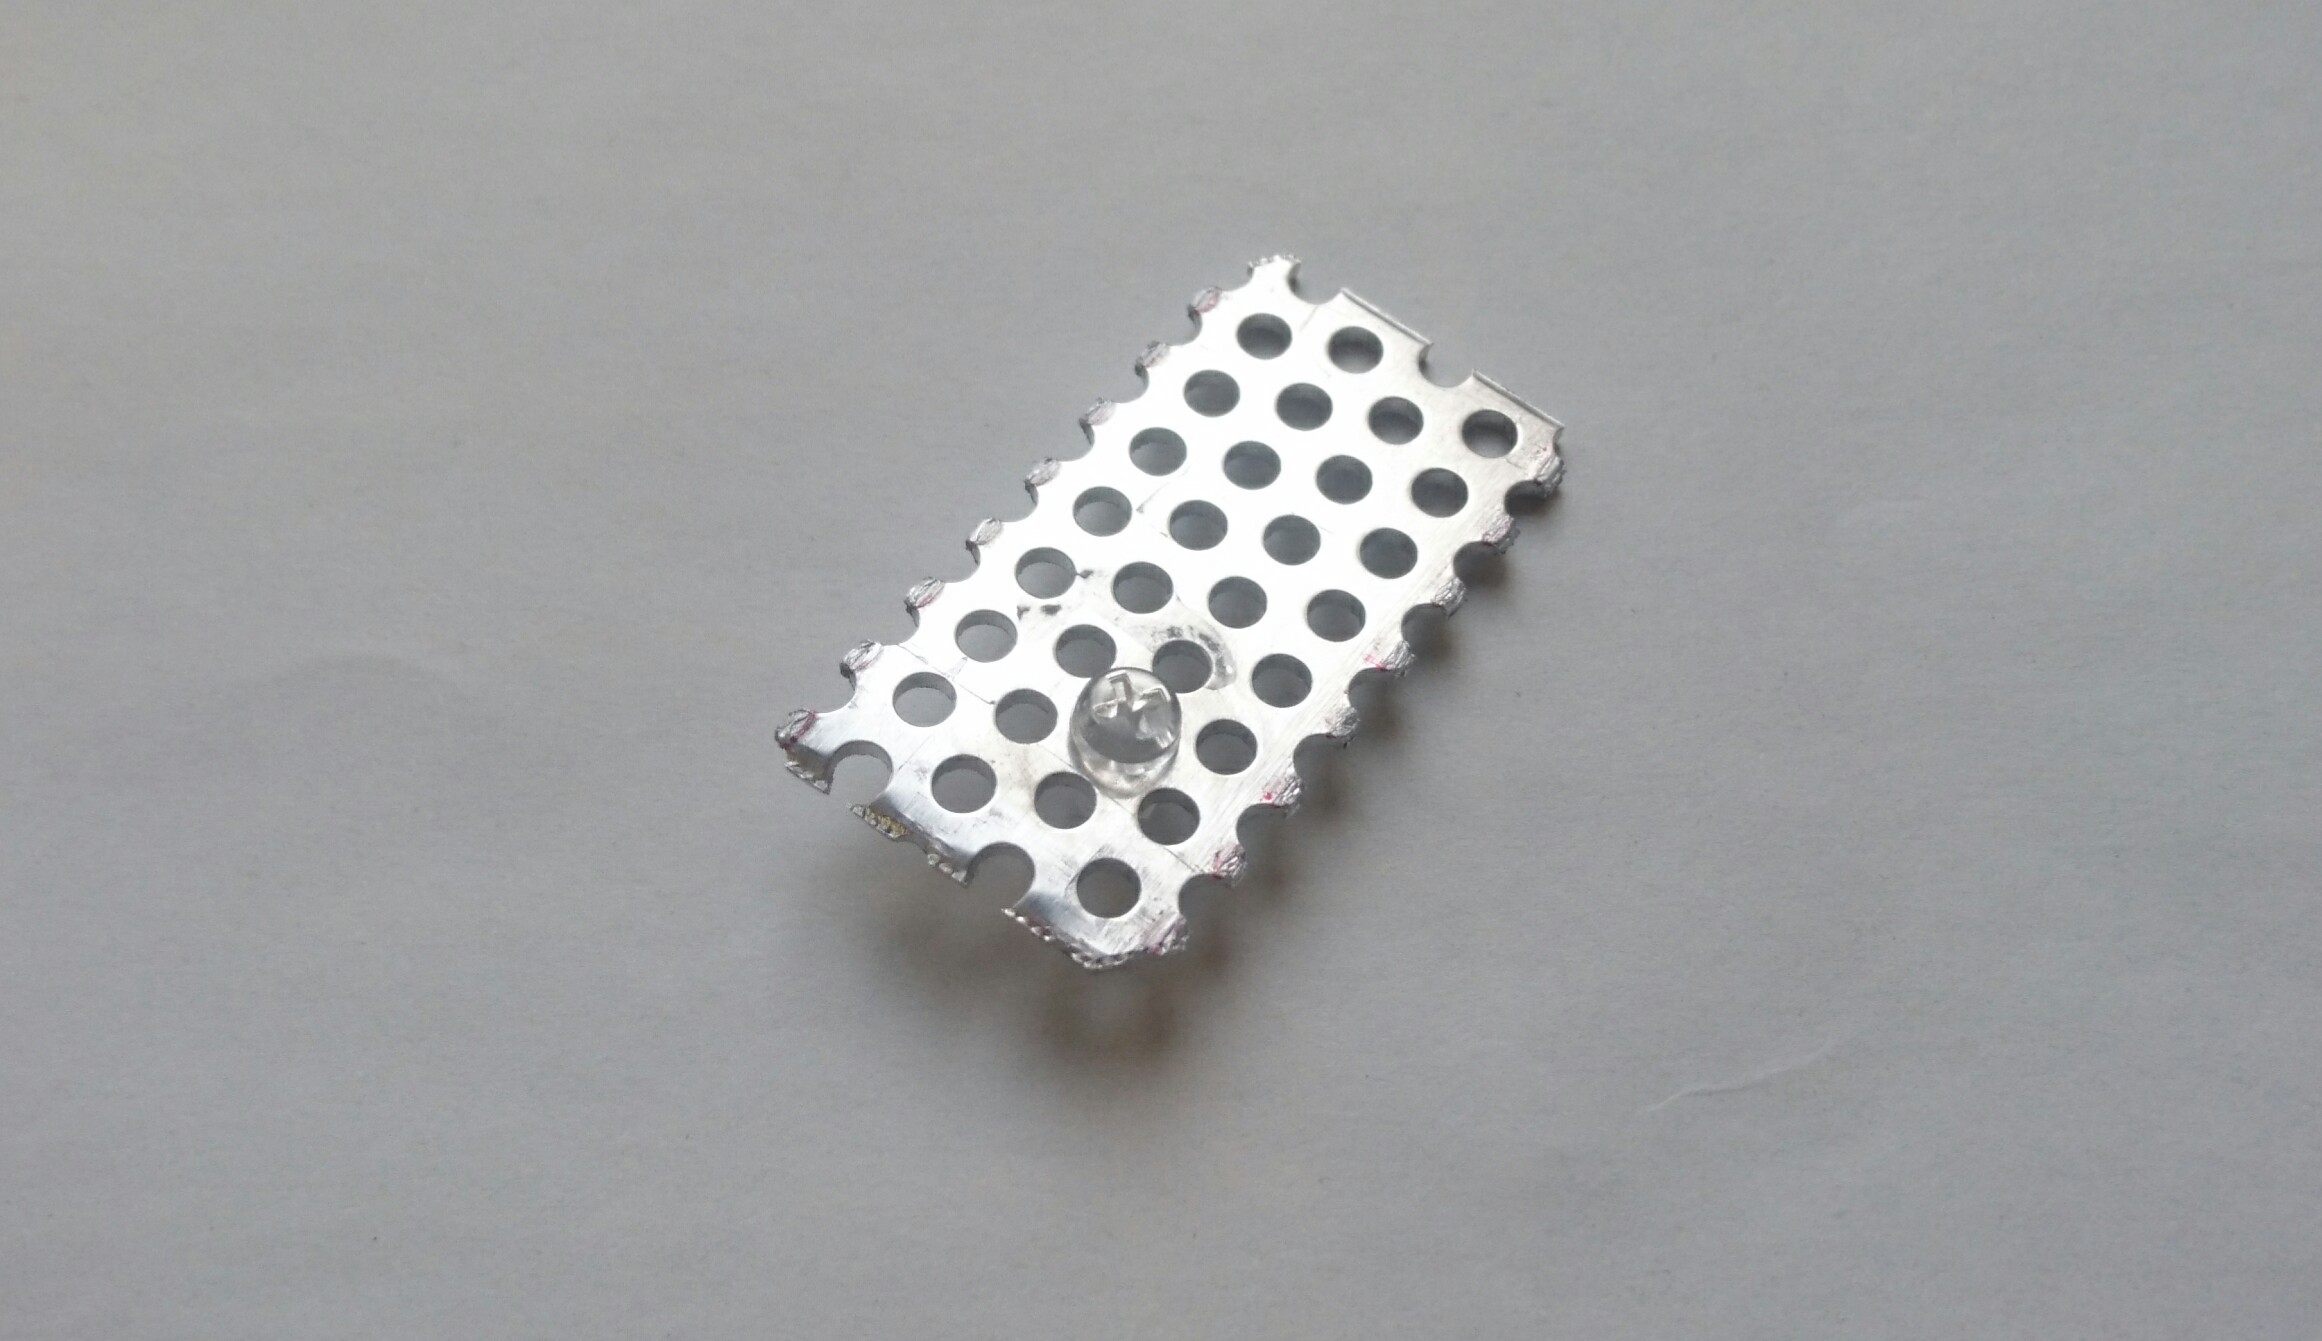
\includegraphics[width=50mm]{hi-to}
    \end{center}
  \caption{ヒートシンク}
 \label{fig:hi-to}
\end{figure}
\subsubsection{通信エラー確認用のLEDの取り付け}
RX220マイコンに図\ref{fig:led}のLEDを取り付け,通信エラーが発生した時に光るように
プログラムした.
\begin{figure}[H]
  \begin{center}
    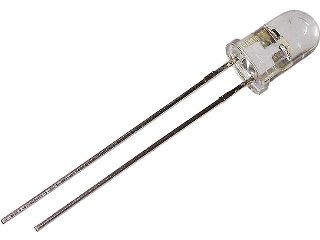
\includegraphics[width=50mm]{led}
    \end{center}
  \caption{5mm 砲弾型LED}
 \label{fig:led}
\end{figure}
\begin{figure}[H]
  \begin{center}
    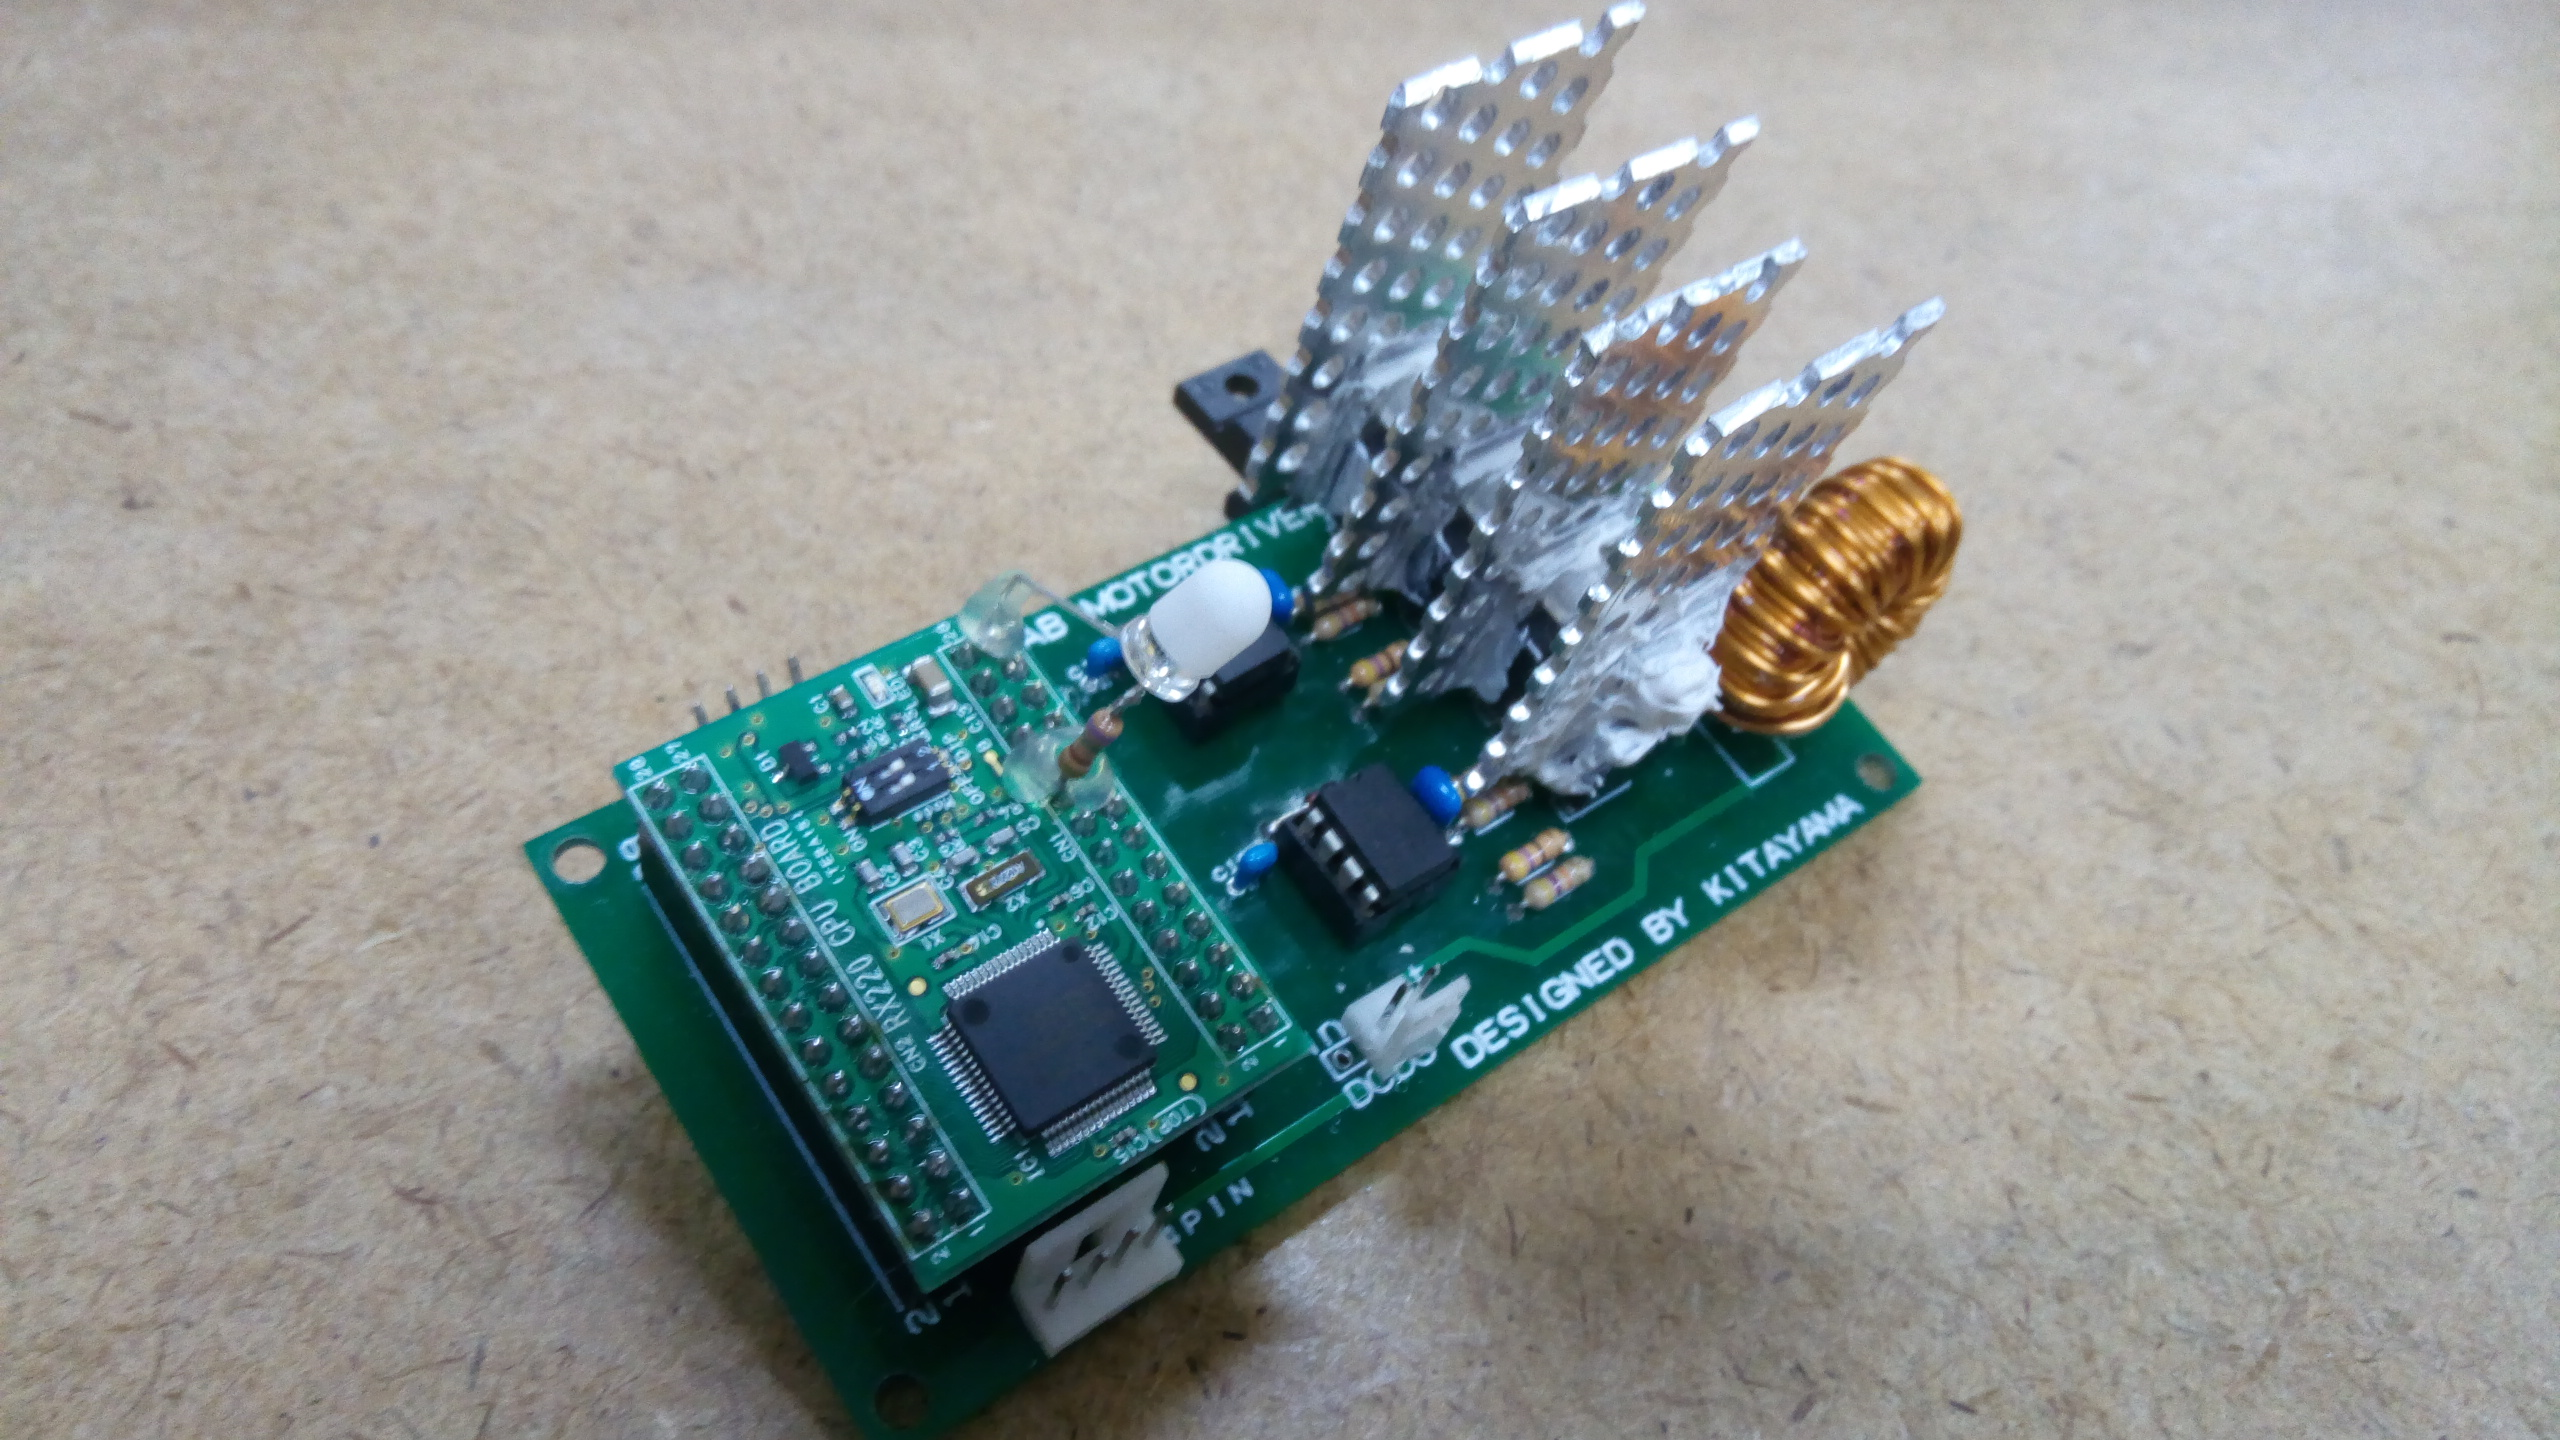
\includegraphics[width=150mm]{shin_driver}
    \end{center}
  \caption{改善後のITOLAB MOTORDRIVER}
 \label{fig:shin_driver}
\end{figure}
\begin{figure}[H]
  \begin{center}
    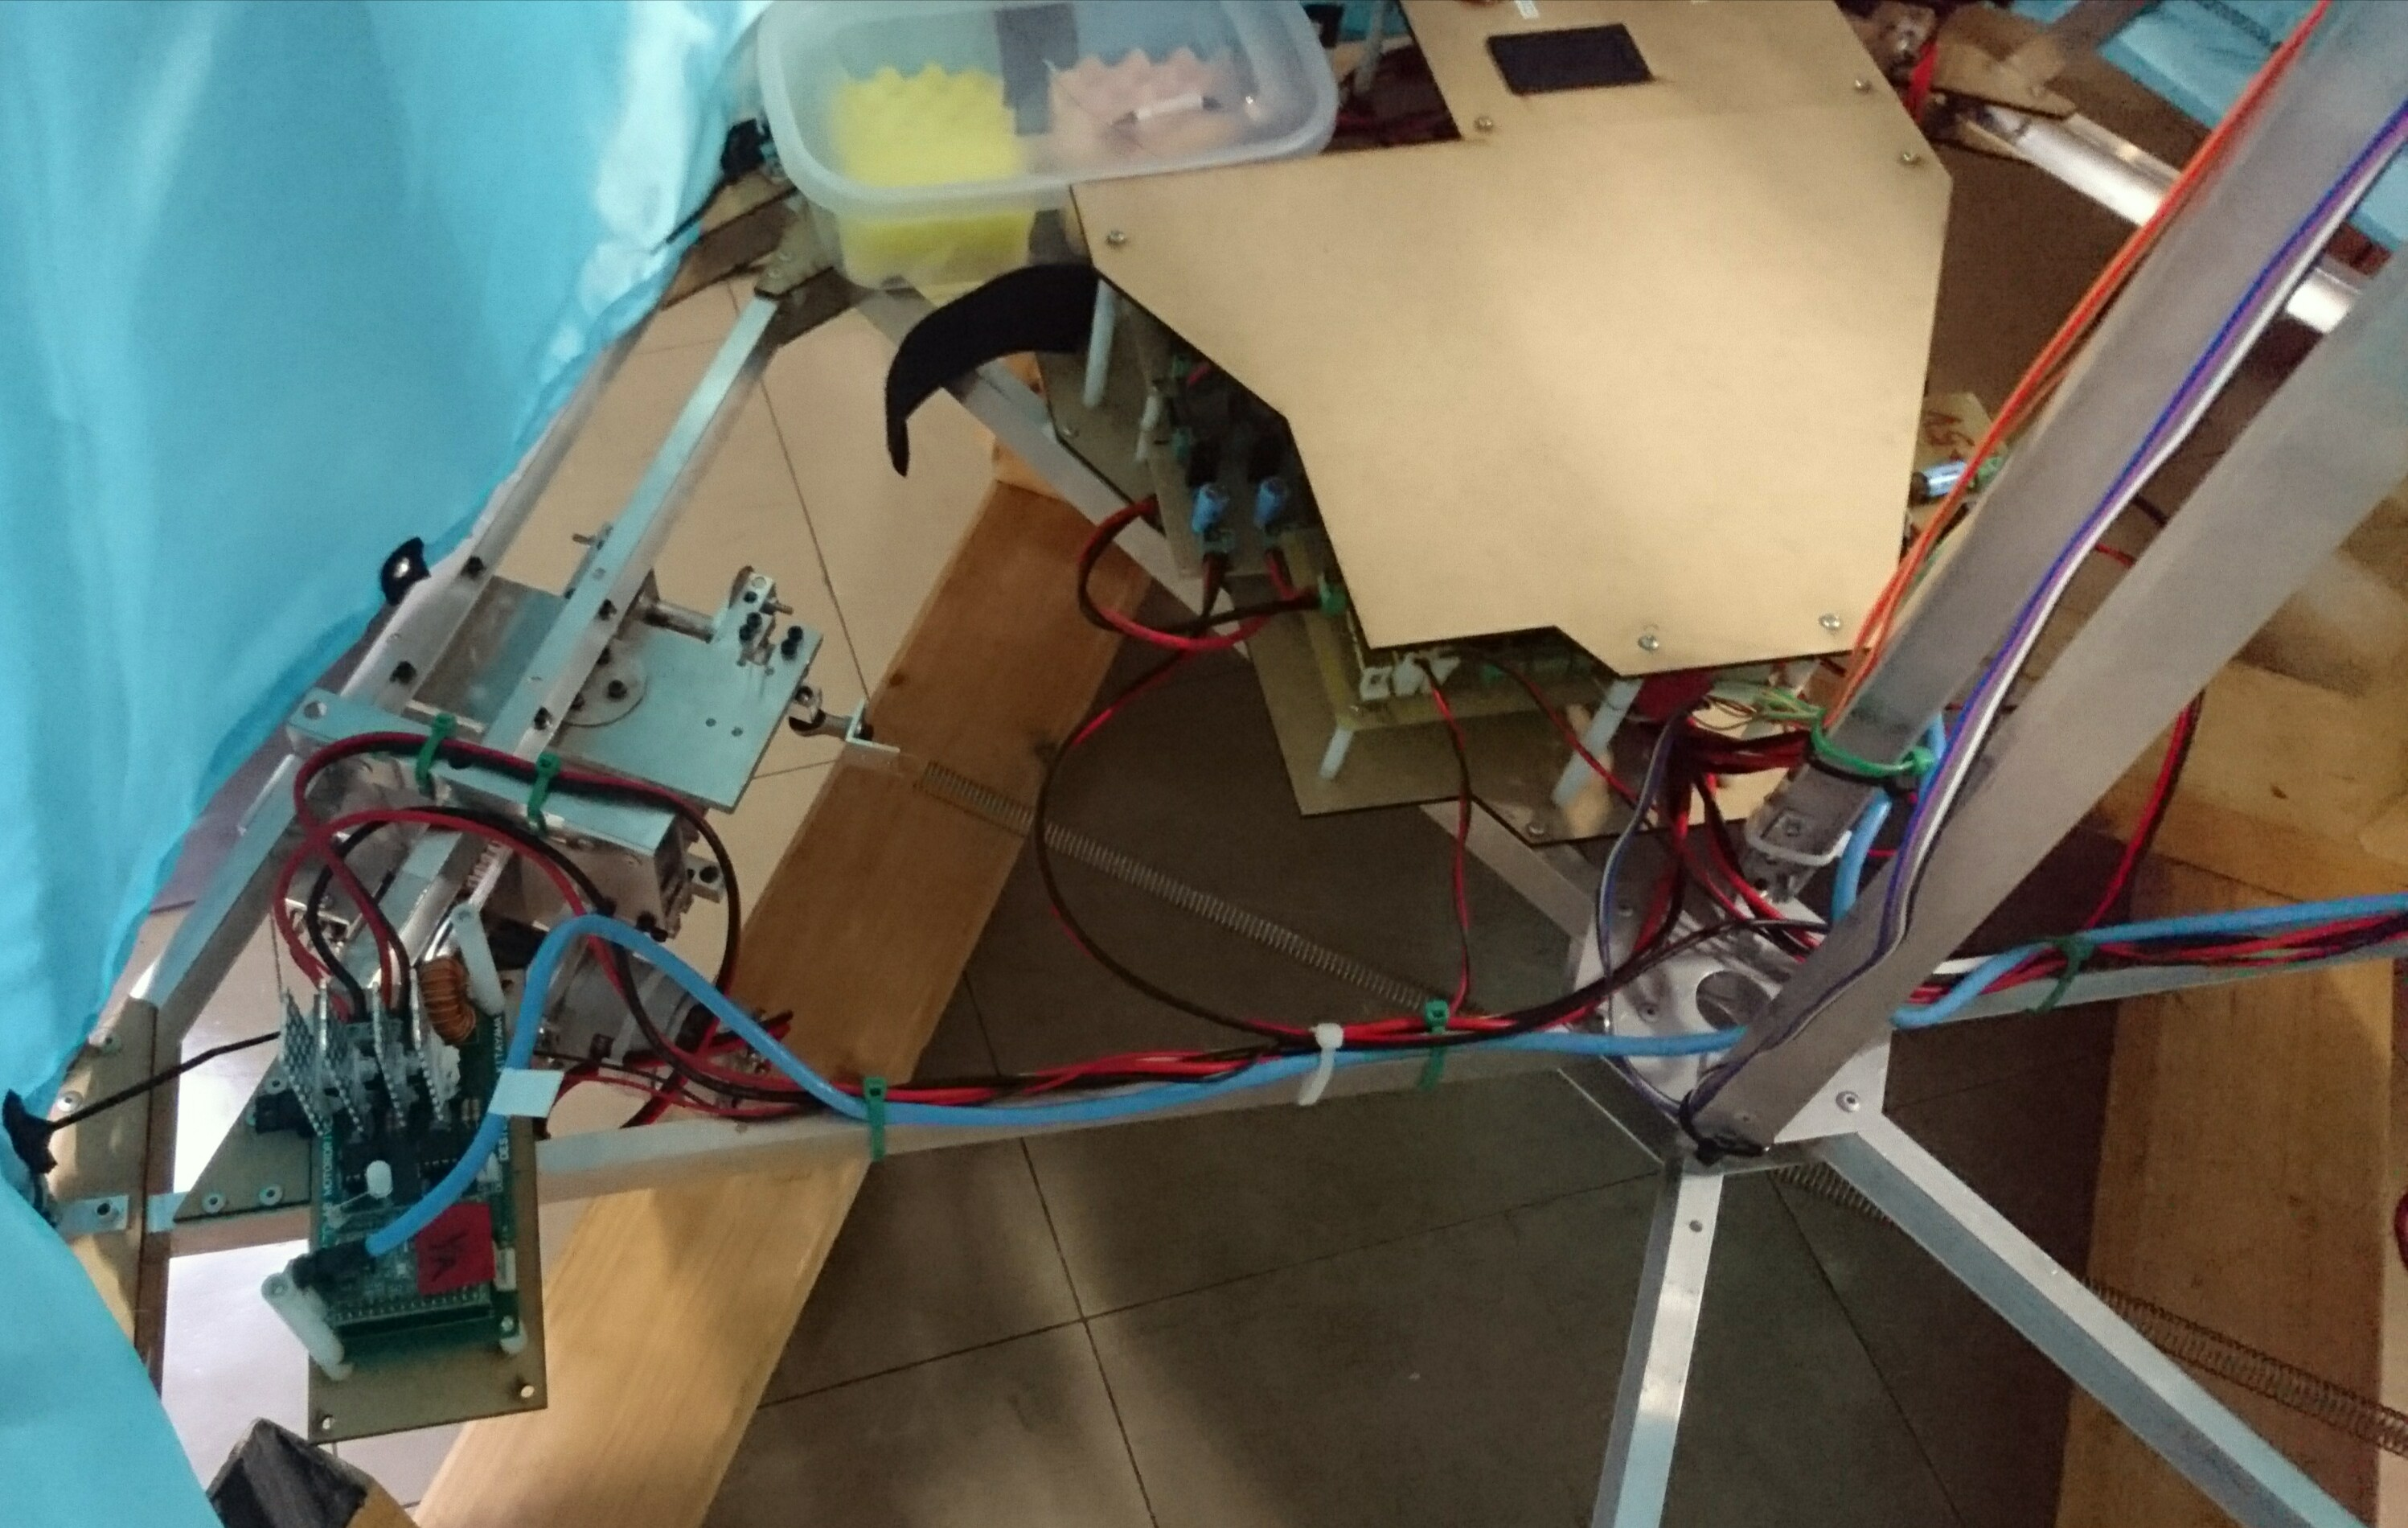
\includegraphics[width=150mm]{robotuke}
    \end{center}
  \caption{ロボットに取り付けたITOLAB MOTORDRIVER}
 \label{fig:robotuke}
\end{figure}

\section{ITOLAB MOTORDRIVER使用結果}
ロボットの最大移動速度を5.83m/sにするために,回転数を1114rpmに設定した.しかし,
電流制限プログラムを入れたために,目標の1114rpmに達せず,700rpmまでとなった.

また,地区大会時に図\ref{fig:teishi}のように1台のロボットのモータが動作
しなくなった.試合後には動作したので,原因を調べたが原因を発見できず,モータドライバ
の不具合も発見できなかった.
\begin{figure}[H]
  \begin{center}
    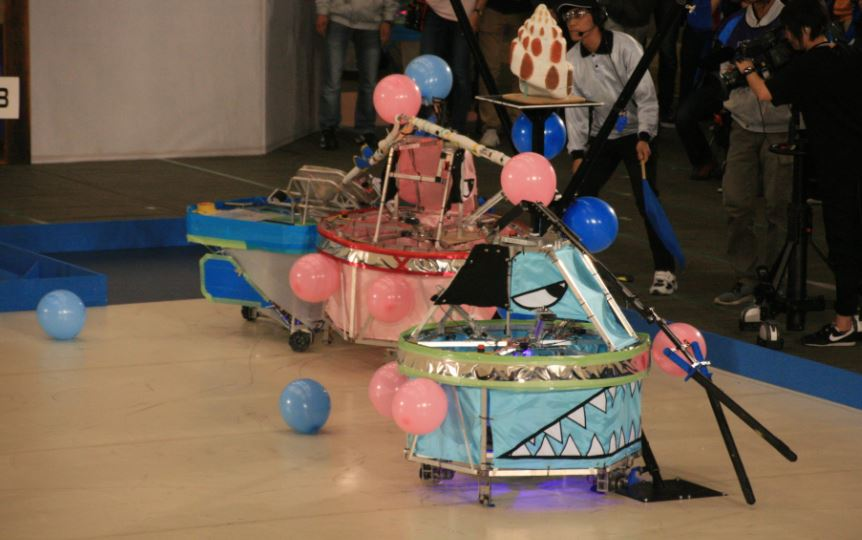
\includegraphics[width=150mm]{teishi}
    \end{center}
  \caption{停止したロボット}
 \label{fig:teishi}
\end{figure}
